% =================================================================================================
% = ///////////////////////////////////////////////////////////////////////////////////////////// =
% = ///                                                                                       /// =
% = /// ABNTEX - UTP                                                                          /// =
% = ///                                                                                       /// =
% = ///////////////////////////////////////////////////////////////////////////////////////////// =
% =================================================================================================
% -------------------------------------------------------------------------------------------------
% - Author: Chauã Queirolo
% - Data:   01/10/2024
% -------------------------------------------------------------------------------------------------
\documentclass[
    12pt
    ,oneside
    ,a4paper
    ,chapter=TITLE
    ,section=TITLE
    ,sumario=abnt-6027-2012]{abntex2}

% Carrega o pacote da abnt com as adapatções para normas da Tuiuti
\usepackage{packages/abnt-UTP}
\usepackage{amssymb}
\usepackage{booktabs}
\usepackage{forest}

% =================================================================================================
% -------------------------------------------------------------------------------------------------
% -                                                                                               -
% - INFORMAÇÕES GERAIS                                                                            -
% -                                                                                               -
% -------------------------------------------------------------------------------------------------
% =================================================================================================

% Informações para CAPA e FOLHA DE ROSTO
\titulo{Ferramenta Baseada em Linguagem de Domínio Específico para o Apoio ao Ensino de Autômatos 
    Finitos com Simulação Visual Interativa}

\autor{João Thomaz Vieira \\ Klaus Siegfried Beckmann}

\orientador{Prof. Diógenes Cogo Furlan}

\preambulo{Trabalho de Conclusão de Curso apresentado ao curso de Bacharelado em Ciência da
Computação da Faculdade de Ciências Exatas e de Tecnologia da Universidade Tuiuti do Paraná,
como requisito à obtenção ao grau de Bacharel.}

\instituicao{Universidade Tuiuti do Paraná}
\local{Curitiba}
\data{\the\year}

% =================================================================================================
% -------------------------------------------------------------------------------------------------
% -                                                                                               -
% - DOCUMENTO                                                                                     -
% -                                                                                               -
% -------------------------------------------------------------------------------------------------
% =================================================================================================
\begin{document}

% =================================================================================================
% -------------------------------------------------------------------------------------------------
% - ELEMENTOS PRÉ-TEXTUAIS                                                                        -
% -------------------------------------------------------------------------------------------------
% =================================================================================================

% -------------------------------------------------------------------------------------------------
% Cria a capa e a folha de rosto
\imprimircapa
\imprimirfolhaderosto

%!!!!!!!!!!!!!!!!!!!!!!!!!!!!!!!!!!!!!!!!!!!!!!!!!!!!!!!!!!!!!!!!!!!!!!!!!!!!!!!!!!!!!!!!!!!!!!!!!!
\begin{agradecimentos}
    Agradecemos a Manoel Gomes, o eterno Caneta Azul, cujo meme nos acompanhou
    nos momentos mais difíceis desta jornada acadêmica. Sua obra, de profundidade
    imensurável, foi a inspiração diária que nos deu forças para continuar.
\end{agradecimentos}

% Resumo do trabalho
\begin{resumo}
    O ensino de autômatos finitos em cursos de Ciência da Computação enfrenta dificuldades
    relacionadas à abstração dos conceitos teóricos, uma vez que as ferramentas existentes adotam
    abordagens exclusivamente visuais, sem oferecer representação textual formal, versionamento ou
    diagnósticos de erro precisos. Este trabalho propõe o desenvolvimento de uma ferramenta
    educacional composta por uma Linguagem de Domínio Específico (DSL) textual para a descrição 
    declarativa de Autômatos Finitos Determinísticos (AFD) e Não-Determinísticos (AFN), acompanhada
    de um compilador que realiza análise léxica, sintática e semântica, fornecendo mensagens de erro
    com indicação de localização e natureza do problema. A ferramenta integra ainda uma interface
    gráfica interativa que renderiza visualmente o autômato descrito e anima o processo de simulação
    passo a passo, destacando os estados e transições percorridos durante o reconhecimento de
    cadeias de entrada. A validação do protótipo é realizada por meio de testes com autômatos
    clássicos da literatura, incluindo casos com erros propositais para avaliar a qualidade dos
    diagnósticos gerados. Espera-se que a ferramenta contribua para a compreensão prática do
    funcionamento de autômatos finitos, conectando a teoria de autômatos à prática de compiladores
    em um único instrumento educacional.

    % O comando \palavraschave inclui automáticamente o ponto final
    \palavraschave{Autômatos Finitos; Linguagem de Domínio Específico; Compiladores; 
        Simulação Visual; Ensino de Computação}
\end{resumo}


% -------------------------------------------------------------------------------------------------
% Listas de ilustrações, tabelas, siglas, etc.
% - Inclua apenas as listas dos elementos que serão utilizados no trabalho.
% - A lista de símbolos e siglas devem ser editadas manualmente
\listadefiguras
% \listadegraficos
\listadetabelas
% \listadequadros
% \listadecodigos
% \listadealgoritmos


% Lista de siglas
% - As siglas deve ser organizadas em ORDEM ALFABÉTICA
% - Inclua apenas as siglas que aparecem no trabalho
\begin{siglas}
    \item[AFD]   Autômato Finito Determinístico
    \item[AFN]   Autômato Finito Não-Determinístico
    \item[AST]   Árvore Sintática Abstrata
    \item[BNF]   Forma de Backus-Naur
    \item[DSL]   Linguagem de Domínio Específico
    \item[EBNF]  Forma de Backus-Naur Estendida
\end{siglas}


% Lista de símbolos
\begin{simbolos}
    \item[$\Sigma$]                   Alfabeto
    \item[$\Sigma^*$]                 Conjunto de todas as palavras sobre $\Sigma$
    \item[$\varepsilon$]              Palavra vazia
    \item[$|w|$]                      Comprimento da palavra $w$
    \item[$\varnothing$]              Conjunto vazio
    \item[$\in$]                      Pertence a
    \item[$\notin$]                   Não pertence a
    \item[$\subseteq$]                Subconjunto
    \item[$\cup$]                     União
    \item[$\cap$]                     Interseção
    \item[$\mathcal{P}(Q)$]           Conjunto das partes de $Q$
    \item[$L^*$]                      Fecho de Kleene da linguagem $L$
    \item[$\to$]                      Regra de produção
    \item[$\Rightarrow$]              Derivação direta
    \item[$\Rightarrow^*$]            Derivação em zero ou mais passos
    \item[$\delta$]                   Função de transição
    \item[$\hat{\delta}$]             Função de transição estendida a cadeias
    \item[$L(M)$]                     Linguagem reconhecida pelo autômato $M$
    \item[$L(G)$]                     Linguagem gerada pela gramática $G$
\end{simbolos}

% Criação do sumário do trabalho
\sumario

% =================================================================================================
% -------------------------------------------------------------------------------------------------
% - ELEMENTOS TEXTUAIS                                                                            -
% -------------------------------------------------------------------------------------------------
% =================================================================================================

% Reinicia a numeração das páginas
\textual

% -------------------------------------------------------------------------------------------------
% -------------------------------------------------------------------------------------------------
% 1. INTRODUÇÃO
% -------------------------------------------------------------------------------------------------
% -------------------------------------------------------------------------------------------------
\chapter{Introdução}
\label{cap:introducao}

O ensino de Teoria da Computação, em especial o conteúdo de autômatos finitos, representa um
desafio recorrente nos cursos de Bacharelado em Ciência da Computação. Conceitos como estados,
transições, alfabetos e reconhecimento de cadeias são abstratos por natureza, e sua compreensão
prática depende fortemente da capacidade do estudante de visualizar e simular o comportamento
das máquinas formais descritas teoricamente em sala de aula.

As ferramentas disponíveis atualmente para apoiar esse aprendizado, como o JFLAP
\cite{rodger2006jflap}, adotam uma abordagem exclusivamente visual baseada em arrastar e soltar,
na qual o usuário constrói o autômato posicionando estados e conectando transições com o \textit{mouse}.
Embora essa abordagem seja útil para ilustrar conceitos, ela apresenta limitações relevantes: a
descrição do autômato não é textual, o que dificulta o versionamento e o compartilhamento dos
modelos; não há validação formal da estrutura com mensagens de erro claras e localizadas; e o
estudante que comete um erro na construção não recebe um diagnóstico preciso do problema.

Diante desse cenário, este trabalho propõe o desenvolvimento de uma ferramenta educacional que
adota uma abordagem diferente. A solução consiste em uma Linguagem de Domínio Específico (DSL)
textual para a descrição declarativa de Autômatos Finitos Determinísticos (AFD) e
Não-Determinísticos (AFN), acompanhada de um compilador que realiza análise léxica, sintática e
semântica, fornecendo mensagens de erro com indicação precisa da localização e da natureza do
problema. A ferramenta integra ainda uma interface gráfica interativa que renderiza visualmente
o autômato descrito e anima o processo de simulação passo a passo, destacando os estados e
transições percorridos durante o reconhecimento de cadeias de entrada.

Um aspecto adicional de relevância é que a própria ferramenta, por ser construída com técnicas
reais de compilação, funciona como um exemplo prático dos conceitos que o estudante está
aprendendo, conectando a teoria de autômatos à prática de compiladores em um único instrumento
educacional. A ausência de uma ferramenta que integre descrição textual formal, validação com
diagnósticos claros e simulação visual interativa justifica o desenvolvimento deste trabalho,
que busca preencher essa lacuna com uma solução unificada e pedagogicamente orientada.

O objetivo geral deste trabalho é desenvolver uma ferramenta educacional baseada em uma
Linguagem de Domínio Específico para apoiar o ensino de autômatos finitos, com simulação visual
interativa. Para atingir esse objetivo, definem-se os seguintes objetivos específicos:

\begin{alineas}
    \item projetar uma DSL textual com sintaxe própria para a descrição declarativa de AFDs e
    AFNs, com a gramática formalizada em notação BNF/EBNF;
    \item implementar um compilador para a DSL com análise léxica, sintática e semântica,
    construindo uma Árvore Sintática Abstrata (AST) e fornecendo mensagens de erro com indicação
    de localização e natureza do problema;
    \item desenvolver um simulador capaz de processar cadeias de entrada sobre os autômatos
    descritos, determinando aceitação ou rejeição e registrando o caminho percorrido;
    \item construir uma interface gráfica interativa que renderize o autômato e anime a simulação
    passo a passo, permitindo ao usuário controlar a velocidade e navegar entre os passos;
    \item validar o protótipo por meio de testes com autômatos clássicos da literatura, incluindo
    casos com erros propositais para avaliar a qualidade dos diagnósticos gerados.
\end{alineas}

Este trabalho está organizado como segue.
O Capítulo~\ref{cap:automatos} apresenta os conceitos teóricos de autômatos finitos e linguagens
formais.
O Capítulo~\ref{cap:conceitos-compiladores} aborda linguagens de domínio específico e as fases de compilação.
O Capítulo~\ref{cap:relacionados} discute as ferramentas relacionadas e suas limitações.
O Capítulo~\ref{cap:projeto} descreve o projeto da DSL, sua sintaxe e gramática.
O Capítulo~\ref{cap:implementacao} detalha a implementação do compilador e da interface gráfica.
O Capítulo~\ref{cap:resultados} apresenta os testes e os resultados obtidos.
Por fim, o Capítulo~\ref{cap:conclusao} apresenta as considerações finais e trabalhos futuros.

% -------------------------------------------------------------------------------------------------
% -------------------------------------------------------------------------------------------------
% 2. Autômatos Finitos e Linguagens Formais (funcamentação teórica)
% -------------------------------------------------------------------------------------------------
% -------------------------------------------------------------------------------------------------
\chapter{Autômatos Finitos e Linguagens Formais}
\label{cap:automatos}
Este capítulo apresenta os fundamentos teóricos necessários à compreensão dos autômatos finitos
e das linguagens regulares, formalismos que constituem o objeto central da ferramenta proposta
neste trabalho. Inicia-se com os conceitos básicos de linguagens formais
(Seção~\ref{sec:linguagens-formais}) e gramáticas (Seção~\ref{sec:gramaticas-formais}),
seguindo-se a formalização dos autômatos finitos determinísticos (Seção~\ref{sec:afd}) e
não-determinísticos (Seção~\ref{sec:afn}). Por fim, demonstra-se a equivalência entre ambos os
modelos (Seção~\ref{sec:equivalencia}), resultado que justifica o uso de qualquer um deles na
descrição de linguagens regulares.

\section{Conceitos Fundamentais de Linguagens Formais}
\label{sec:linguagens-formais}
O estudo dos autômatos finitos exige a compreensão prévia de algumas estruturas matemáticas
elementares: conjuntos, alfabetos, palavras e linguagens. Esta seção apresenta tais conceitos de
forma sistemática, fixando a notação e a terminologia adotadas nos capítulos subsequentes.

Um \textbf{conjunto} é uma coleção de elementos, que podem ser de qualquer natureza, como
números, letras, símbolos ou mesmo outros conjuntos. Para indicar que um elemento $a$ pertence a um conjunto
$C$, escreve-se $a \in C$; o símbolo $\notin$ denota a relação inversa. Por exemplo, dado
$C = \{a, b, c\}$, tem-se $a \in C$ e $d \notin C$. Conjuntos podem ser finitos ou infinitos; no
segundo caso, é usual o emprego de reticências para indicar a continuação dos elementos, como em
$\mathbb{Z} = \{\ldots, -2, -1, 0, 1, 2, \ldots\}$. O conjunto que não contém qualquer elemento é
denominado \textbf{conjunto vazio} e é representado pelo símbolo $\varnothing$ \cite{sipser2012}.

A partir desta noção de conjunto, define-se a primeira estrutura específica da teoria das
linguagens formais: o alfabeto. Um \textbf{alfabeto} é um conjunto finito e não vazio de símbolos,
representado, por convenção, pela letra grega $\Sigma$ \cite{sipser2012}. Os elementos de um
alfabeto são denominados símbolos ou letras. Por exemplo, $\Sigma_1 = \{0, 1\}$ é o alfabeto
binário, enquanto $\Sigma_2 = \{a, b, c, \ldots, z\}$ corresponde ao alfabeto latino minúsculo. A
exigência de finitude é fundamental, pois garante que os autômatos, definidos nas seções
seguintes, possam manipular o alfabeto de forma efetiva; a não vacuidade, por sua vez, assegura
que sempre haja ao menos um símbolo disponível para a formação de palavras
\cite{vieira2006,diverio2011}.

Sobre um alfabeto $\Sigma$, define-se uma \textbf{palavra} (ou cadeia) como uma sequência finita
de símbolos pertencentes a $\Sigma$, escritos de forma justaposta e sem separadores. O comprimento
de uma palavra $w$, denotado por $|w|$, corresponde ao número de símbolos que a compõem. A palavra
de comprimento zero, denominada \textbf{palavra vazia}, é representada pelo símbolo $\varepsilon$
\cite{sipser2012}. O conjunto de todas as palavras que podem ser formadas sobre $\Sigma$,
incluindo a palavra vazia, é denotado por $\Sigma^*$. Assim, para $\Sigma = \{a, b\}$, tem-se
$\Sigma^* = \{\varepsilon, a, b, aa, ab, ba, bb, aaa, \ldots\}$, conjunto que é sempre infinito e
enumerável \cite{vieira2006}.

Estabelecidas as noções de alfabeto e palavra, é possível definir o objeto central deste trabalho:
a linguagem. Uma \textbf{linguagem formal} sobre um alfabeto $\Sigma$ é qualquer subconjunto de
$\Sigma^*$, ou seja, qualquer conjunto de palavras formadas a partir dos símbolos de $\Sigma$
\cite{sipser2012,vieira2006}. Linguagens podem ser finitas, como $L_1 = \{a, ab, abb\}$, ou
infinitas, como $L_2 = \{a^n b^n \mid n \geq 1\}$, que contém todas as palavras compostas por uma
sequência de $a$'s seguida de igual número de $b$'s. A maior parte das linguagens de interesse
teórico e prático é infinita, o que motiva o desenvolvimento de mecanismos formais, como
gramáticas e autômatos, capazes de descrevê-las de maneira finita.

Por serem conjuntos, as linguagens admitem as operações usuais de \textbf{união},
\textbf{interseção} e \textbf{diferença}. Além dessas, três operações específicas, derivadas da
estrutura sequencial das palavras, desempenham papel central na teoria
\cite{vieira2006,diverio2011}. A \textbf{concatenação} de duas palavras
$x = a_1 a_2 \cdots a_m$ e $y = b_1 b_2 \cdots b_n$ produz a palavra
$xy = a_1 a_2 \cdots a_m b_1 b_2 \cdots b_n$; em particular, $w\varepsilon = \varepsilon w = w$
para qualquer palavra $w$, o que faz de $\varepsilon$ o elemento neutro dessa operação. A
concatenação estende-se naturalmente a linguagens: dadas $L_1$ e $L_2$, define-se
$L_1 L_2 = \{xy \mid x \in L_1 \text{ e } y \in L_2\}$. Por fim, o \textbf{fecho de Kleene} de uma
linguagem $L$, denotado por $L^*$, corresponde ao conjunto de todas as palavras obtidas pela
concatenação de zero ou mais elementos de $L$, isto é, $L^* = \bigcup_{n \in \mathbb{N}} L^n$,
onde $L^0 = \{\varepsilon\}$ e $L^n = L^{n-1} L$ para $n \geq 1$. Essas operações constituem a
base para a especificação concisa de linguagens, recurso amplamente explorado nas expressões
regulares e gramáticas estudadas nas seções seguintes.

\section{Gramáticas Formais}
\label{sec:gramaticas-formais}
Conforme observado na seção anterior, a maior parte das linguagens de interesse prático é
infinita, o que torna inviável descrevê-las pela enumeração explícita de suas palavras. Faz-se
necessário, portanto, um mecanismo finito capaz de gerar todas as palavras de uma linguagem.
Entre os formalismos propostos para esse fim, as \textbf{gramáticas} ocupam posição de destaque,
tanto pelo seu poder expressivo quanto pela estreita relação com os autômatos estudados nas
seções subsequentes \cite{vieira2006,lewis1998}.

Uma gramática descreve uma linguagem por meio de um conjunto finito de \textbf{regras de
produção}, que indicam como certas sequências de símbolos podem ser substituídas por outras.
Nessa estrutura, distinguem-se dois tipos de símbolos: os \textbf{terminais}, que compõem o
alfabeto da linguagem gerada e aparecem nas palavras finais, e os \textbf{não-terminais} (ou
\textbf{variáveis}), símbolos auxiliares que servem de intermediários no processo de geração e
não fazem parte das palavras produzidas \cite{lewis1998,sipser2012}. A geração de uma palavra
inicia-se sempre a partir de uma variável especial, denominada \textbf{símbolo inicial} (ou
variável de partida), e prossegue pela aplicação sucessiva das regras até que reste apenas uma
sequência de terminais.

Formalmente, uma \textbf{gramática} é uma quádrupla $G = (V, \Sigma, R, S)$, na qual
\cite{vieira2006,lewis1998}:
\begin{itemize}
    \item $V$ é um conjunto finito de variáveis (símbolos não-terminais);
    \item $\Sigma$ é um alfabeto de símbolos terminais, com $V \cap \Sigma = \varnothing$;
    \item $R$ é um conjunto finito de \textbf{regras de produção}, cada uma escrita na forma
          $\alpha \to \beta$, em que $\alpha, \beta \in (V \cup \Sigma)^*$ e o lado esquerdo
          $\alpha$ contém ao menos uma variável;
    \item $S \in V$ é a variável de partida.
\end{itemize}

A aplicação de uma regra $\alpha \to \beta \in R$ a uma cadeia de variáveis e terminais produz
uma nova cadeia pela substituição de uma ocorrência de $\alpha$ por $\beta$. Essa relação de
substituição direta é denotada por $\Rightarrow$: dadas $u, v \in (V \cup \Sigma)^*$, escreve-se
$u \Rightarrow v$ quando existem $x, y \in (V \cup \Sigma)^*$ e uma regra
$\alpha \to \beta \in R$ tais que $u = x\alpha y$ e $v = x\beta y$ \cite{lewis1998}. Em outras
palavras, $x$ e $y$ representam o trecho da cadeia que permanece inalterado, enquanto a
subcadeia $\alpha$, situada entre eles, é trocada por $\beta$. A título de exemplo, dada a regra
$A \to ab$ e a cadeia $cAd$, tem-se $cAd \Rightarrow cabd$, identificando-se $x = c$,
$\alpha = A$, $y = d$ e $\beta = ab$.

A aplicação sucessiva de regras, isto é, o fecho reflexivo e transitivo de $\Rightarrow$, é
denotada por $\Rightarrow^*$. A \textbf{linguagem gerada} pela gramática $G$ é o conjunto de
todas as palavras formadas exclusivamente por terminais que podem ser obtidas a partir do
símbolo inicial: $L(G) = \{ w \in \Sigma^* \mid S \Rightarrow^* w \}$
\cite{vieira2006,sipser2012}.

A título de ilustração, considere a gramática $G = (\{S\}, \{a, b\}, R, S)$, em que
$R = \{S \to aSb,\ S \to \varepsilon\}$. Partindo do símbolo inicial $S$, é possível obter, por
exemplo, a palavra $aabb$ por meio da seguinte derivação:
\begin{align*}
    S &\Rightarrow aSb   && \text{(aplicação da regra } S \to aSb\text{)} \\
      &\Rightarrow aaSbb && \text{(aplicação da regra } S \to aSb\text{)} \\
      &\Rightarrow aabb  && \text{(aplicação da regra } S \to \varepsilon\text{)}
\end{align*}
A estrutura dessa derivação pode ser visualizada por meio de uma \textbf{árvore de derivação},
representada na Figura~\ref{fig:arvore-derivacao}, na qual a raiz corresponde ao símbolo inicial,
os nós internos representam as variáveis substituídas e as folhas correspondem aos terminais que
compõem a palavra gerada \cite{sipser2012}.

\begin{figure}[h]
    \centering
    \begin{forest}
        for tree={
            math content,
            l sep=14pt,
            s sep=18pt,
            inner sep=2pt
        }
        [S
            [a]
            [S
                [a]
                [S [\varepsilon]]
                [b]
            ]
            [b]
        ]
    \end{forest}
    \caption{Árvore de derivação da palavra $aabb$ na gramática $G$}
    \label{fig:arvore-derivacao}
    \fonte{Os autores (\the\year)}
\end{figure}

De modo geral, cada aplicação da regra $S \to aSb$ acrescenta um $a$ à esquerda e um $b$ à
direita do símbolo $S$, enquanto a regra $S \to \varepsilon$ encerra a derivação eliminando a
variável remanescente. Conclui-se que $L(G) = \{a^n b^n \mid n \geq 0\}$, linguagem que, conforme
será discutido adiante, não pode ser gerada por nenhum mecanismo mais restrito que uma gramática
livre de contexto \cite{lewis1998,sipser2012}.

Restrições impostas sobre a forma das regras de produção dão origem a diferentes classes de
gramáticas e, consequentemente, a diferentes classes de linguagens. Essa estratificação,
conhecida como \textbf{Hierarquia de Chomsky}, organiza as linguagens em quatro categorias
(irrestritas, sensíveis ao contexto, livres de contexto e regulares), cada uma associada a um
modelo computacional específico \cite{vieira2006,lewis1998}. O Quadro~\ref{quad:chomsky} sintetiza
essa classificação, evidenciando a forma das regras de produção admitidas em cada classe e o
modelo computacional que reconhece a linguagem correspondente.

\begin{table}[h]
    \centering
    \caption{Hierarquia de Chomsky}
    \label{quad:chomsky}
    \small
    \setlength{\tabcolsep}{5pt}
    \begin{tabular}{c l l l}
        \toprule
        \textbf{Tipo} & \textbf{Classe de Linguagem}    & \textbf{Forma das Regras}                & \textbf{Modelo Computacional}    \\
        \midrule
        0             & Recursivamente enumeráveis      & $\alpha \to \beta$                       & Máquina de Turing                \\
        1             & Sensíveis ao contexto           & $\alpha A \beta \to \alpha \gamma \beta$ & Autômato linearmente limitado    \\
        2             & Livres de contexto              & $A \to \gamma$                           & Autômato com pilha               \\
        3             & Regulares                       & $A \to aB$ ou $A \to a$                  & Autômato finito                  \\
        \bottomrule
    \end{tabular}
    \fonte{Adaptado de \citeonline{vieira2006} e \citeonline{lewis1998}}
\end{table}

As gramáticas regulares (Tipo 3), em particular, geram exatamente a classe das linguagens
reconhecidas pelos autômatos finitos, formalismo apresentado nas próximas seções.

\section{Autômato Finito Determinístico}
\label{sec:afd}
Conforme indicado ao final da seção anterior, as gramáticas regulares (Tipo 3 da Hierarquia de
Chomsky) descrevem exatamente a classe das linguagens reconhecidas pelo modelo computacional
mais simples: o autômato finito. Esta seção apresenta a formalização do \textbf{autômato finito
determinístico} (AFD), modelo que serve como ponto de partida para o estudo dos reconhecedores
de linguagens regulares e que constitui o objeto central da ferramenta proposta neste trabalho.

Intuitivamente, um AFD é uma máquina abstrata composta por um número finito de \textbf{estados},
interligados por \textbf{transições} rotuladas com símbolos de um alfabeto. A máquina inicia sua
operação em um estado especial, denominado \textbf{estado inicial}, e processa uma cadeia de
entrada lendo seus símbolos um a um, da esquerda para a direita. A cada símbolo lido, o autômato
transita para um novo estado, conforme determinado pela rotulação das arestas. Encerrado o
processamento da cadeia, se o autômato encontrar-se em um dos estados designados como
\textbf{estados finais} (ou de aceitação), diz-se que a cadeia foi \textbf{aceita}; caso
contrário, é \textbf{rejeitada} \cite{hopcroft2006,sipser2012}. O termo
\textit{determinístico} reflete a característica de que, para cada combinação de estado atual e
símbolo de entrada, existe uma única transição possível.

Formalmente, um \textbf{autômato finito determinístico} é uma quíntupla
$M = (Q, \Sigma, \delta, q_0, F)$, na qual \cite{hopcroft2006,sipser2012}:
\begin{itemize}
    \item $Q$ é um conjunto finito de estados;
    \item $\Sigma$ é um alfabeto finito de símbolos de entrada;
    \item $\delta : Q \times \Sigma \to Q$ é a \textbf{função de transição}, que associa a cada
          par formado por um estado e um símbolo o estado para o qual o autômato transita;
    \item $q_0 \in Q$ é o estado inicial;
    \item $F \subseteq Q$ é o conjunto de estados finais (ou de aceitação).
\end{itemize}

A função $\delta$ descreve o comportamento do autômato ao ler um único símbolo. Para representar
o processamento de uma cadeia inteira, define-se sua extensão recursiva
$\hat{\delta} : Q \times \Sigma^* \to Q$, dada por \cite{hopcroft2006}:
\begin{align*}
    \hat{\delta}(q, \varepsilon) &= q, \\
    \hat{\delta}(q, wa)          &= \delta(\hat{\delta}(q, w), a),
\end{align*}
em que $w \in \Sigma^*$ e $a \in \Sigma$. A função estendida indica, portanto, o estado em que
o autômato se encontra após processar uma cadeia $w$ a partir do estado $q$. A
\textbf{linguagem reconhecida} (ou aceita) por um AFD $M$, denotada $L(M)$, é o conjunto de
todas as cadeias que conduzem o autômato, partindo do estado inicial, a algum estado de
aceitação:
\[
    L(M) = \{\, w \in \Sigma^* \mid \hat{\delta}(q_0, w) \in F \,\}.
\]
As linguagens reconhecidas por algum AFD são denominadas \textbf{linguagens regulares}
\cite{sipser2012}.

A representação gráfica de um AFD é feita por meio de um \textbf{diagrama de estados}, no qual
os estados são representados por círculos, as transições por arestas rotuladas com os símbolos
correspondentes, o estado inicial é apontado por uma seta sem origem e os estados de aceitação
são marcados com círculos duplos. A título de exemplo, considere o AFD apresentado na
Figura~\ref{fig:afd-exemplo}, que reconhece a linguagem das cadeias sobre $\{0, 1\}$ que contêm
$01$ como subcadeia \cite{hopcroft2006}.

\begin{figure}[h]
    \centering
    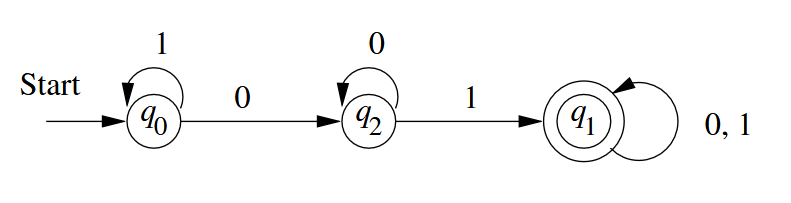
\includegraphics[width=0.75\textwidth]{img/automato_finito_deterministico.png}
    \caption{AFD que reconhece cadeias contendo $01$ como subcadeia}
    \label{fig:afd-exemplo}
    \fonte{\citeonline{hopcroft2006}}
\end{figure}

Formalmente, o autômato da Figura~\ref{fig:afd-exemplo} é descrito como
$M = (Q, \Sigma, \delta, q_0, F)$, em que $Q = \{q_0, q_1, q_2\}$, $\Sigma = \{0, 1\}$,
$F = \{q_1\}$ e a função $\delta$ é dada pelas transições $\delta(q_0, 0) = q_2$,
$\delta(q_0, 1) = q_0$, $\delta(q_2, 0) = q_2$, $\delta(q_2, 1) = q_1$, $\delta(q_1, 0) = q_1$ e
$\delta(q_1, 1) = q_1$. Cada estado codifica uma informação distinta sobre o histórico da
leitura: $q_0$ indica que ainda não foi lido nenhum $0$ (ou que o último símbolo lido foi $1$),
$q_2$ indica que o último símbolo lido foi $0$ e $q_1$ indica que a subcadeia $01$ já foi
identificada \cite{hopcroft2006}.

A título de ilustração, ao processar a cadeia $1101$, o autômato realiza a sequência de
transições $q_0 \xrightarrow{1} q_0 \xrightarrow{1} q_0 \xrightarrow{0} q_2 \xrightarrow{1}
q_1$, atingindo o estado de aceitação $q_1$, de modo que a cadeia é aceita. Por outro lado, ao
processar a cadeia $111$, o autômato permanece em $q_0$ ao longo de toda a leitura e a cadeia é
rejeitada por não terminar em estado final. Verifica-se que $L(M)$ corresponde exatamente ao
conjunto das cadeias sobre $\{0, 1\}$ que contêm a subcadeia $01$, em conformidade com a
especificação informal apresentada.

\section{Autômato Finito Não-Determinístico}
\label{sec:afn}
O autômato finito determinístico apresentado na seção anterior caracteriza-se por possuir, para
cada combinação de estado e símbolo de entrada, uma única transição definida. Em diversas
situações, no entanto, é mais natural descrever um reconhecedor permitindo que, em certos
estados, mais de uma transição esteja disponível para o mesmo símbolo, ou ainda que, em outros,
não haja qualquer transição definida \cite{hopcroft2006,sipser2012}. Tal flexibilidade dá origem
ao \textbf{autômato finito não-determinístico} (AFN), modelo que, embora distinto em
comportamento, reconhece a mesma classe de linguagens que os AFDs.

A diferença essencial em relação ao AFD reside na natureza da função de transição. Enquanto, em
um AFD, a aplicação de $\delta$ a um par estado-símbolo retorna um único estado, em um AFN ela
retorna um \textbf{conjunto} de estados, possivelmente vazio. Isso significa que, ao processar
um símbolo a partir de um dado estado, o AFN pode prosseguir por qualquer um dos estados
indicados (caso haja mais de um) ou travar (caso o conjunto seja vazio). Intuitivamente,
imagina-se que o autômato investiga simultaneamente todas as escolhas possíveis: o caminho
computacional que, ao final da leitura, atinge um estado de aceitação determina a aceitação da
cadeia, mesmo que outros caminhos tenham travado ou terminado em estados não-finais
\cite{sipser2012}.

Formalmente, um \textbf{autômato finito não-determinístico} é uma quíntupla
$N = (Q, \Sigma, \delta, q_0, F)$, na qual \cite{hopcroft2006,sipser2012}:
\begin{itemize}
    \item $Q$ é um conjunto finito de estados;
    \item $\Sigma$ é um alfabeto finito de símbolos de entrada;
    \item $\delta : Q \times \Sigma \to \mathcal{P}(Q)$ é a \textbf{função de transição}, que
          associa a cada par estado-símbolo um subconjunto de $Q$, sendo $\mathcal{P}(Q)$ o
          conjunto das partes de $Q$;
    \item $q_0 \in Q$ é o estado inicial;
    \item $F \subseteq Q$ é o conjunto de estados finais.
\end{itemize}

A extensão da função de transição a cadeias, denotada $\hat{\delta}$, é definida recursivamente
de modo análogo ao caso determinístico, levando em consideração que cada passo pode produzir
múltiplos estados \cite{hopcroft2006}:
\begin{align*}
    \hat{\delta}(q, \varepsilon) &= \{q\}, \\
    \hat{\delta}(q, wa)          &= \bigcup_{p \in \hat{\delta}(q, w)} \delta(p, a),
\end{align*}
em que $w \in \Sigma^*$ e $a \in \Sigma$. A função estendida indica, portanto, o conjunto de
todos os estados em que o autômato pode encontrar-se após processar a cadeia $w$ a partir do
estado $q$. A \textbf{linguagem aceita} por um AFN $N$, denotada $L(N)$, é o conjunto das
cadeias para as quais existe ao menos um caminho computacional terminando em estado de
aceitação:
\[
    L(N) = \{\, w \in \Sigma^* \mid \hat{\delta}(q_0, w) \cap F \neq \varnothing \,\}.
\]
Em outras palavras, basta que uma das possíveis sequências de transições conduza a um estado
final para que a cadeia seja aceita \cite{hopcroft2006,sipser2012}.

A título de exemplo, considere o AFN apresentado na Figura~\ref{fig:afn-exemplo}, que reconhece
a linguagem das cadeias sobre $\{0, 1\}$ que terminam em $01$ \cite{hopcroft2006}.

\begin{figure}[h]
    \centering
    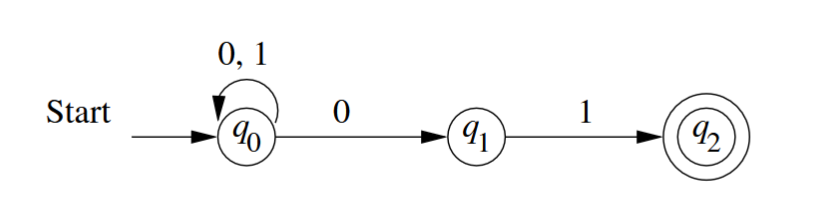
\includegraphics[width=0.75\textwidth]{img/automato_finito_nao_deterministico.png}
    \caption{AFN que reconhece cadeias terminadas em $01$}
    \label{fig:afn-exemplo}
    \fonte{\citeonline{hopcroft2006}}
\end{figure}

Esse autômato é descrito formalmente como
$N = (\{q_0, q_1, q_2\}, \{0, 1\}, \delta, q_0, \{q_2\})$, em que a função de transição é dada
por $\delta(q_0, 0) = \{q_0, q_1\}$, $\delta(q_0, 1) = \{q_0\}$, $\delta(q_1, 1) = \{q_2\}$ e
os demais valores correspondem ao conjunto vazio. As duas características que evidenciam o
não-determinismo ficam aparentes nessa especificação: o estado $q_0$ admite duas transições
distintas para o símbolo $0$ (o autômato pode permanecer em $q_0$ ou avançar para $q_1$),
enquanto os estados $q_1$ e $q_2$ apresentam transições ausentes para certos símbolos.

Para ilustrar o funcionamento, considere o processamento da cadeia $001$. Partindo de
$\hat{\delta}(q_0, \varepsilon) = \{q_0\}$, calcula-se sucessivamente
$\hat{\delta}(q_0, 0) = \{q_0, q_1\}$, $\hat{\delta}(q_0, 00) = \{q_0, q_1\}$ e
$\hat{\delta}(q_0, 001) = \{q_0, q_2\}$. Como $q_2 \in F$, a cadeia é aceita. Por outro lado, ao
processar a cadeia $010$, obtém-se ao final $\hat{\delta}(q_0, 010) = \{q_0, q_1\}$, conjunto que
não contém o estado final $q_2$, de modo que a cadeia é rejeitada.

Embora o não-determinismo confira maior flexibilidade aparente na descrição de linguagens,
demonstra-se que toda linguagem reconhecida por um AFN também pode ser reconhecida por algum
AFD \cite{hopcroft2006,sipser2012}. Esse resultado, fundamentado na chamada \textbf{construção
de subconjuntos}, é apresentado na seção seguinte e justifica o fato de ambos os modelos
definirem exatamente a mesma classe de linguagens: as linguagens regulares.

\section{Equivalência entre AFD e AFN}
\label{sec:equivalencia}
Embora o autômato finito não-determinístico ofereça maior flexibilidade na descrição de
linguagens, demonstra-se que essa flexibilidade não amplia a classe de linguagens reconhecíveis.
Mais precisamente, vale o seguinte resultado central da teoria dos autômatos: uma linguagem $L$
é reconhecida por algum AFD se, e somente se, é reconhecida por algum AFN
\cite{hopcroft2006,sipser2012}. Em outras palavras, AFDs e AFNs são modelos
\textbf{equivalentes em poder de reconhecimento}, ainda que possam diferir significativamente em
número de estados e em facilidade de projeto.

A demonstração desse resultado é constituída por duas direções. A primeira, e mais imediata,
consiste em observar que todo AFD pode ser interpretado como um AFN: basta tomar a função de
transição do AFD e, para cada par estado-símbolo, considerar o conjunto unitário formado pelo
único destino existente. Como o AFN resultante simula passo a passo o AFD original, ambos
reconhecem a mesma linguagem \cite{hopcroft2006}. A segunda direção, conhecida como
\textbf{construção de subconjuntos} (\textit{subset construction}), é menos trivial e fornece um
procedimento algorítmico para converter qualquer AFN em um AFD equivalente.

A construção de subconjuntos parte da seguinte ideia: em um AFN, após ler uma cadeia $w$, o
autômato pode encontrar-se em qualquer um dos estados pertencentes a $\hat{\delta}(q_0, w)$. O
AFD equivalente, por sua vez, simula esse comportamento mantendo, em cada um de seus estados,
\textit{o conjunto de estados do AFN} em que a computação poderia estar a partir da leitura
realizada até aquele momento. Os estados do AFD são, portanto, subconjuntos do conjunto de
estados do AFN \cite{hopcroft2006}.

Formalmente, dado um AFN $N = (Q_N, \Sigma, \delta_N, q_0, F_N)$, constrói-se o AFD equivalente
$D = (Q_D, \Sigma, \delta_D, q_{0,D}, F_D)$ por meio das seguintes definições
\cite{hopcroft2006}:
\begin{itemize}
    \item $Q_D = \mathcal{P}(Q_N)$, ou seja, cada estado do AFD é um subconjunto de estados do
          AFN;
    \item $q_{0,D} = \{q_0\}$, isto é, o estado inicial do AFD corresponde ao conjunto que
          contém apenas o estado inicial do AFN;
    \item $F_D = \{\, S \in Q_D \mid S \cap F_N \neq \varnothing \,\}$, ou seja, um subconjunto
          é considerado estado de aceitação do AFD se contiver ao menos um estado de aceitação
          do AFN;
    \item $\delta_D(S, a) = \bigcup_{p \in S} \delta_N(p, a)$ para cada $S \in Q_D$ e cada
          $a \in \Sigma$, isto é, a transição do AFD a partir de um subconjunto $S$ é a união
          das transições que o AFN executaria a partir de cada estado em $S$.
\end{itemize}

Embora $\mathcal{P}(Q_N)$ contenha $2^{|Q_N|}$ elementos no caso geral, em geral apenas uma
pequena fração desses subconjuntos é efetivamente alcançável a partir do estado inicial. Na
prática, o procedimento é aplicado de forma incremental: parte-se de $\{q_0\}$ e, a cada passo,
computam-se as transições para os subconjuntos ainda não explorados, até que nenhum novo
subconjunto seja gerado. A correção da construção é assegurada pelo seguinte teorema, demonstrado
em \citeonline{hopcroft2006}: \textit{uma linguagem $L \subseteq \Sigma^*$ é reconhecida por
algum AFN se, e somente se, é reconhecida por algum AFD}.

A título de ilustração, considere novamente o AFN da Figura~\ref{fig:afn-exemplo}, que reconhece
as cadeias sobre $\{0, 1\}$ terminadas em $01$. Aplicando a construção de subconjuntos a esse
autômato, parte-se do estado inicial $\{q_0\}$ e calculam-se as transições conforme o
procedimento descrito. Tem-se, por exemplo, $\delta_D(\{q_0\}, 0) = \delta_N(q_0, 0) =
\{q_0, q_1\}$ e $\delta_D(\{q_0\}, 1) = \{q_0\}$. Continuando o processo, geram-se sucessivamente
os demais subconjuntos alcançáveis até que o AFD se estabilize. O resultado final é apresentado
na Figura~\ref{fig:afd-construido}.

\begin{figure}[h]
    \centering
    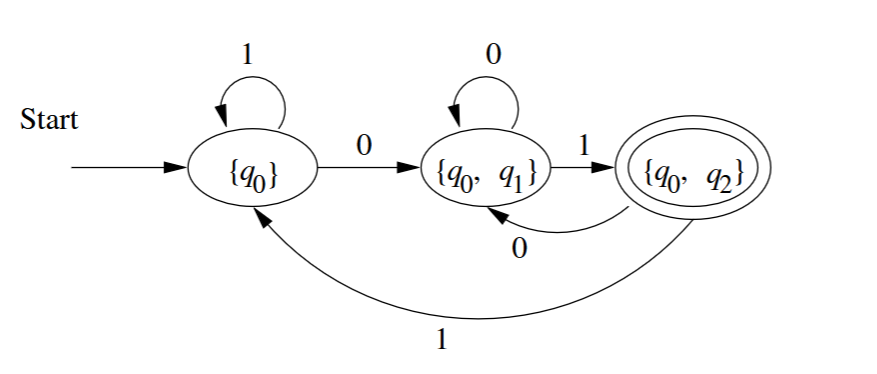
\includegraphics[width=0.85\textwidth]{img/dfa_construida_a_partir_da_nfa.png}
    \caption{AFD construído a partir do AFN da Figura~\ref{fig:afn-exemplo} pela construção de subconjuntos}
    \label{fig:afd-construido}
    \fonte{\citeonline{hopcroft2006}}
\end{figure}

Observa-se que o AFD resultante possui apenas três estados ($\{q_0\}$, $\{q_0, q_1\}$ e
$\{q_0, q_2\}$), ainda que o conjunto das partes de $Q_N$ contivesse oito subconjuntos possíveis.
O estado $\{q_0, q_2\}$ é o único estado de aceitação, pois é o único subconjunto acessível que
contém $q_2$, estado final do AFN de origem. Verifica-se diretamente que $L(D) = L(N)$, isto é,
o AFD construído reconhece exatamente a mesma linguagem do AFN de partida \cite{hopcroft2006}.

Vale observar, por fim, que, no pior caso, a construção de subconjuntos pode produzir um AFD
com $2^n$ estados a partir de um AFN com $n$ estados, ainda que, na prática, o número de estados
acessíveis costume ser comparável ao do AFN original \cite{hopcroft2006}. Essa diferença,
contudo, não altera a equivalência em poder expressivo: ambos os modelos definem exatamente a
classe das linguagens regulares.

\section{Representações de Autômatos}
\label{sec:representacoes_automatos}
A definição formal de autômato finito como uma quíntupla, apresentada nas seções anteriores, é
suficiente para caracterizar matematicamente o objeto, mas não é necessariamente a forma mais
prática de descrevê-lo no dia a dia. Na literatura e em ferramentas educacionais, são utilizadas
três representações distintas e complementares, cada uma adequada a um propósito específico
\cite{hopcroft2006,sipser2012}. Esta seção apresenta essas representações, evidenciando as
vantagens e limitações de cada uma.

A primeira forma é a \textbf{notação formal}, em que o autômato é descrito explicitamente como a
quíntupla $M = (Q, \Sigma, \delta, q_0, F)$, listando-se cada um de seus componentes. Trata-se
da representação mais precisa e desambígua, sendo indispensável em demonstrações matemáticas e
em provas de equivalência. Por outro lado, sua leitura direta é trabalhosa: a função de
transição $\delta$, em particular, costuma ser apresentada como uma enumeração de pares
$\delta(q, a) = q'$, que rapidamente se torna extensa à medida que cresce o número de estados
\cite{hopcroft2006}.

A segunda forma é o \textbf{diagrama de estados}, já utilizado nas Figuras~\ref{fig:afd-exemplo}
e~\ref{fig:afn-exemplo} das seções anteriores. Nessa representação, cada estado corresponde a um
nó (círculo simples para estados comuns ou círculo duplo para estados de aceitação), as
transições são arestas rotuladas com os símbolos do alfabeto, e o estado inicial é apontado por
uma seta sem origem \cite{hopcroft2006,sipser2012}. O diagrama de estados é o formato preferido
em contextos didáticos e em ferramentas como o JFLAP \cite{rodger2006jflap}, pois permite que o
leitor reconheça visualmente padrões como ciclos, estados de absorção e simetrias. Sua principal
limitação é a dificuldade de manipulação textual: o diagrama é uma imagem e, portanto, não pode
ser facilmente versionado, comparado ou processado por ferramentas automatizadas.

A terceira forma é a \textbf{tabela de transição}, que organiza a função $\delta$ em uma matriz
bidimensional cujas linhas correspondem aos estados e cujas colunas correspondem aos símbolos do
alfabeto \cite{hopcroft2006}. A Tabela~\ref{tab:tabela-transicao-afd} ilustra essa representação
para o AFD da Figura~\ref{fig:afd-exemplo}, que reconhece cadeias contendo $01$ como subcadeia.
A seta ($\rightarrow$) marca o estado inicial e o asterisco ($*$) destaca o estado de
aceitação, conforme convenção adotada por \citeonline{hopcroft2006}.

\begin{table}[h]
    \centering
    \caption{Tabela de transição do AFD que reconhece cadeias contendo $01$}
    \label{tab:tabela-transicao-afd}
    \begin{tabular}{c c c}
        \toprule
                                    & \textbf{0} & \textbf{1} \\
        \midrule
        $\rightarrow q_0$           & $q_2$      & $q_0$      \\
        $\phantom{\rightarrow} q_2$ & $q_2$      & $q_1$      \\
        $* q_1$                     & $q_1$      & $q_1$      \\
        \bottomrule
    \end{tabular}
    \fonte{Adaptado de \citeonline{hopcroft2006}}
\end{table}

A leitura da tabela é direta: cada célula $(q, a)$ contém o estado $\delta(q, a)$ para o qual o
autômato transita ao ler o símbolo $a$ a partir do estado $q$. Essa representação combina
precisão formal e leitura sistemática, sendo compacta, permitindo verificar facilmente se a
função de transição está completa (no caso do AFD, todas as células devem estar preenchidas) e
sendo particularmente adequada para o processamento programático, pois pode ser diretamente
codificada como uma matriz ou estrutura de dados equivalente \cite{hopcroft2006,sipser2012}.
Para AFNs, a tabela de transição segue o mesmo formato, com a diferença de que cada célula
contém um \textit{conjunto} de estados em vez de um único estado, podendo, inclusive, conter o
conjunto vazio quando não houver transição definida \cite{hopcroft2006}.

As três representações apresentadas (notação formal, diagrama de estados e tabela de transição)
são complementares e equivalentes entre si, descrevendo o mesmo objeto matemático sob
perspectivas distintas. A escolha entre elas depende do contexto de uso: o rigor formal favorece
a notação como quíntupla; a comunicação didática favorece o diagrama; a manipulação computacional
favorece a tabela. A ferramenta proposta neste trabalho explora essa equivalência ao oferecer
uma quarta forma de representação, baseada em uma linguagem de domínio específico textual, que
combina a precisão da notação formal com a estruturação tabular, permitindo simultaneamente a
renderização do diagrama de estados e o processamento programático da descrição.

\section{Simulação de Autômatos}
\label{sec:simulacao_automatos}

A definição formal de um autômato finito, vista nas seções anteriores, descreve sob a forma de
quíntupla os elementos que compõem a máquina, mas não esclarece, por si só, como verificar se
uma cadeia específica é aceita ou rejeitada. Essa verificação, conhecida como
\textbf{simulação}, consiste em executar passo a passo a função de transição $\delta$ a partir
do estado inicial, consumindo cada símbolo da cadeia de entrada e observando se a configuração
final corresponde a um estado de aceitação \cite{hopcroft2006,sipser2012}. Em termos
pedagógicos, a simulação cumpre um papel análogo ao da execução de um programa em uma linguagem
de programação, pois permite que o estudante observe o comportamento do autômato projetado e
confronte-o com o comportamento esperado \cite{morazan2014}.

\citeonline{morazan2014} argumentam que disciplinas introdutórias de linguagens formais,
tradicionalmente, exigem que estudantes projetem máquinas e provem sua correção sem oferecer
mecanismos para experimentar com os artefatos produzidos. Os autores defendem que essa ausência
de retroalimentação imediata contraria a forma como o estudante de Ciência da Computação aprende
a programar, em que compiladores e interpretadores fornecem mensagens de erro e advertências
durante o desenvolvimento. A consequência observada é que estudantes inexperientes submetem com
frequência soluções incorretas, mesmo para exercícios relativamente simples, e dedicam esforço
a tentativas de prova de correção sobre projetos defeituosos \cite{morazan2014}. Para mitigar
esse problema, os autores propõem que a teoria da computação seja ensinada com ferramentas
capazes de \textit{construir} computações, isto é, ambientes em que a descrição formal possa
ser traduzida em uma representação executável e submetida a testes.

Formalmente, simular um AFD $M = (Q, \Sigma, \delta, q_0, F)$ sobre uma cadeia $w = a_1 a_2
\dots a_n \in \Sigma^*$ corresponde a calcular a sequência de configurações $q_0, q_1, \dots,
q_n$, em que $q_i = \delta(q_{i-1}, a_i)$ para $1 \leq i \leq n$. A cadeia $w$ é aceita se, e
somente se, $q_n \in F$ \cite{hopcroft2006}. Para um AFD, a simulação é determinística e
linear: cada símbolo lido conduz a exatamente um próximo estado, de modo que o custo
computacional cresce proporcionalmente ao comprimento da cadeia. Essa propriedade torna o AFD
particularmente adequado para implementações eficientes, pois pode ser realizado por uma
estrutura de dados simples, como uma tabela de transição indexada pelo par (estado, símbolo)
\cite{sipser2012}.

A simulação de um AFN, em contraste, exige tratamento adicional, pois a função de transição
$\delta$ pode levar um mesmo par (estado, símbolo) a um conjunto de estados, e transições
$\varepsilon$ permitem mudança de estado sem consumir símbolos da entrada. Conforme descrito
por \citeonline{morazan2014} ao apresentar a função \textit{apply-sm} da biblioteca FSM, a
simulação de uma máquina não determinística é realizada por meio de uma busca em largura sobre
todos os caminhos possíveis que o autômato pode seguir ao consumir a cadeia. Em cada passo, o
simulador mantém o conjunto de estados alcançáveis e, ao final da entrada, verifica se algum
desses estados pertence ao conjunto de aceitação. Alternativamente, conforme \citeonline{hopcroft2006},
o AFN pode ser convertido previamente em um AFD equivalente pelo algoritmo de construção de
subconjuntos, transferindo a simulação para o caso determinístico ao custo de uma possível
expansão exponencial do número de estados.

Além de produzir um veredito de aceitação ou rejeição, uma ferramenta de simulação útil para o
ensino deve expor o \textit{caminho percorrido} pelo autômato, isto é, a sequência de
configurações intermediárias atravessadas durante o processamento da cadeia. \citeonline{morazan2014}
denominam essa funcionalidade \textit{show-transitions} e destacam sua importância para que o
estudante identifique exatamente em que ponto sua máquina diverge do comportamento esperado.
Essa visualização do \textit{trace} de execução substitui o exercício manual de acompanhar transições
em papel, propenso a erros, por uma observação direta do comportamento da máquina, em
consonância com a prática de depuração comum no desenvolvimento de \textit{software}.

A relevância da simulação ganha ainda mais destaque quando se considera o fenômeno descrito por
\citeonline{morazan2014} de que estudantes, sem ambiente de teste, frequentemente partem para
demonstrações formais sobre projetos incorretos, com perda de tempo e desmotivação como
consequência. Esse argumento é central para o presente trabalho: a ferramenta proposta busca
oferecer simulação visual interativa diretamente acoplada à descrição textual do autômato, de
forma que o estudante possa, a partir de uma única especificação, examinar a estrutura do
diagrama de estados, executar cadeias de teste e acompanhar a evolução das configurações,
recebendo retroalimentação imediata sobre o comportamento da máquina.

Cabe ainda diferenciar dois sentidos do termo simulação que aparecem na literatura. Em sentido
estrito, simular um autômato é executar sua função de transição sobre uma entrada específica,
como descrito acima. Em sentido mais amplo, ferramentas como o JFLAP \cite{rodger2006jflap} e a
biblioteca FSM \cite{morazan2014} oferecem também a possibilidade de \textit{testar} um
autômato com múltiplas cadeias geradas aleatoriamente, comparar duas máquinas quanto à
equivalência de suas linguagens e visualizar transformações construtivas, como a conversão de
AFN em AFD. Essas operações estendem a noção básica de simulação para um conjunto mais rico de
recursos didáticos, ao qual se pode atribuir o termo \textit{ambiente de experimentação}. A
ferramenta proposta neste trabalho posiciona-se nesse espectro, oferecendo, em primeiro plano,
a simulação visual passo a passo de autômatos finitos descritos por meio de uma linguagem de
domínio específico, conforme será detalhado no Capítulo~\ref{cap:conceitos-compiladores}.

\section{Aplicações de Autômatos}
\label{sec:aplicacoes_automatos}

Apesar de serem objetos teóricos, autômatos finitos não são uma abstração restrita ao ambiente
acadêmico. \citeonline{hopcroft2006} destacam que esse modelo computacional sustenta o
funcionamento de diversas categorias de \textit{software} e \textit{hardware} utilizadas no dia a dia, sempre que
um sistema precisa registrar, em um número finito de configurações, a parte relevante de seu
histórico para decidir qual ação tomar diante da próxima entrada. Esta seção apresenta as
principais áreas de aplicação descritas pelos autores e estabelece a ponte entre os conceitos
formais discutidos até aqui e os capítulos seguintes deste trabalho.

\citeonline{hopcroft2006} agrupam as aplicações dos autômatos finitos em quatro grandes
categorias:

\begin{itemize}
    \item \textbf{Projeto e verificação de circuitos digitais.} Sistemas digitais com um número
    finito de estados internos podem ser modelados diretamente como autômatos, permitindo que
    o comportamento do circuito seja descrito de forma rigorosa e verificado antes da
    implementação física. Cada estado do autômato corresponde a uma configuração possível do
    circuito, e cada transição corresponde à resposta do \textit{hardware} a um sinal de entrada
    \cite{hopcroft2006}.

    \item \textbf{Análise léxica de compiladores.} O componente responsável por dividir o
    texto-fonte em unidades léxicas (identificadores, palavras-chave, operadores e literais)
    é tipicamente implementado como um autômato finito. \citeonline{hopcroft2006} ilustram
    esse uso com um autômato cuja função é reconhecer a palavra-chave \texttt{then}: cada
    estado corresponde a um prefixo da palavra (vazio, $t$, $th$, $the$, $then$), e a
    sequência de transições percorrida pela cadeia de entrada determina se o lexema foi
    encontrado. Esse mesmo princípio se generaliza para o reconhecimento de qualquer conjunto
    finito de \textit{tokens} descrito por expressões regulares.

    \item \textbf{Busca de padrões em grandes volumes de texto.} Sistemas que percorrem
    coleções extensas de documentos, páginas \textit{web} ou arquivos em busca de palavras,
    expressões ou padrões mais complexos costumam compilar essas consultas em autômatos
    finitos, executando a varredura em tempo proporcional ao tamanho da entrada
    \cite{hopcroft2006}. Utilitários clássicos do ambiente Unix, como \textit{grep}, e
    bibliotecas modernas de expressões regulares apoiam-se diretamente nessa equivalência
    entre expressões regulares e autômatos finitos.

    \item \textbf{Verificação de sistemas com número finito de estados.} Protocolos de
    comunicação, protocolos criptográficos e outros sistemas reativos podem ser modelados
    como autômatos para que propriedades como ausência de \textit{deadlock}, alcançabilidade
    de estados ou conformidade com uma especificação sejam verificadas automaticamente
    \cite{hopcroft2006}.
\end{itemize}

A presença pervasiva dos autômatos finitos nessas áreas decorre de uma característica central
do modelo: o número fixo de estados permite que sua representação seja implementada com uma
quantidade limitada de recursos, seja como um circuito de \textit{hardware}, seja como uma estrutura
de dados em memória \cite{hopcroft2006}. Esse equilíbrio entre simplicidade e poder expressivo
explica por que o modelo permanece relevante mesmo após décadas de evolução das ferramentas
de \textit{software}.

Para o presente trabalho, a aplicação de maior interesse é a análise léxica, pois constitui o
elo direto entre a teoria dos autômatos finitos e a construção de compiladores e
interpretadores para linguagens de programação. A linguagem de domínio específico proposta
nesta monografia, descrita no Capítulo~\ref{cap:conceitos-compiladores}, será analisada
lexicamente por um autômato finito gerado a partir das regras léxicas da própria linguagem,
em uma aplicação concreta dos conceitos apresentados neste capítulo.

% -------------------------------------------------------------------------------------------------
% -------------------------------------------------------------------------------------------------
% 2. Compiladores e Linguagens de Domínio Específico (funcamentação teórica)
% -------------------------------------------------------------------------------------------------
% -------------------------------------------------------------------------------------------------

\chapter{Conceitos de Compiladores}
\label{cap:conceitos-compiladores}

\section{Análise Léxica}
\label{sec:lexica}

\section{Análise Sintática}
\label{sec:sintatica}

\section{Análise Semântica}
\label{sec:semantica}

\section{AST (Árvore Sintática Abstrata)}
\label{sec:ast}

\section{Linguagens de Domínio Específico (DSL)}
\label{sec:dsl}

\section{Construção de Compiladores (ferramentas)}
\label{sec:contrucao-compiladores}

\section{Diagnóstico de Erros}
\label{sec:diagnostico-erro}

\section{DSL no ensino}
\label{sec:dsl-ensino}

\chapter{Rust}
\label{cap:rust}

% -------------------------------------------------------------------------------------------------
% -------------------------------------------------------------------------------------------------
% -------------------------------------------------------------------------------------------------

% =================================================================================================
% -------------------------------------------------------------------------------------------------
% - ELEMENTOS PÓS-TEXTUAIS                                                                            -
% -------------------------------------------------------------------------------------------------
% =================================================================================================

% Inicia a seção pós-textual
\postextual

% -------------------------------------------------------------------------------------------------
% REFERÊNCIAS BIBLIOGRÁFICAS
% -------------------------------------------------------------------------------------------------

% Carrega o arquivo referencias.bib
\bibliography{referencias}


% -------------------------------------------------------------------------------------------------
% APÊNDICES
% -------------------------------------------------------------------------------------------------
% \apendice[ape:exemplo]{Exemplo de Apêndice}


% -------------------------------------------------------------------------------------------------
% ANEXOS
% -------------------------------------------------------------------------------------------------
% \anexo[ane:exemplo]{Exemplo de Anexo}


\end{document}
